\documentclass[border=4pt]{standalone}
\usepackage{tikz}
\usetikzlibrary{positioning,arrows.meta,fit,calc}
\usepackage{amsmath,amssymb}
\begin{document}
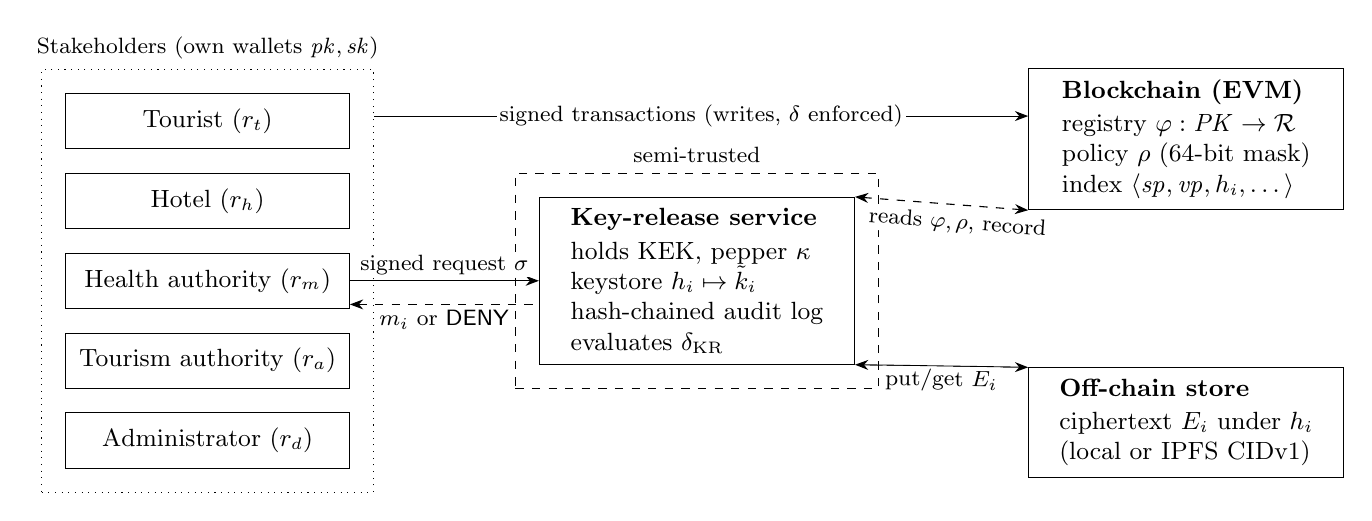
\begin{tikzpicture}[font=\small,>=Stealth,
  ent/.style={draw,minimum width=36mm,minimum height=7mm,align=center},
  box/.style={draw,align=left,inner sep=4pt},
  lab/.style={font=\footnotesize,fill=white,inner sep=1pt}]
% stakeholders
\node[ent] (tour) {Tourist ($r_t$)};
\node[ent,below=3mm of tour] (hotel) {Hotel ($r_h$)};
\node[ent,below=3mm of hotel] (health) {Health authority ($r_m$)};
\node[ent,below=3mm of health] (tauth) {Tourism authority ($r_a$)};
\node[ent,below=3mm of tauth] (admin) {Administrator ($r_d$)};
\node[draw,dotted,inner sep=3mm,fit=(tour)(admin),label={[font=\footnotesize]above:Stakeholders (own wallets $\mathit{pk}, \mathit{sk}$)}] (stake) {};
% key-release service
\node[box,right=24mm of health,minimum width=40mm] (krs) {\textbf{Key-release service}\\[1pt]
  holds $\mathrm{KEK}$, pepper $\kappa$\\
  keystore $h_i \mapsto \tilde{k}_i$\\
  hash-chained audit log\\
  evaluates $\delta_{\mathrm{KR}}$};
\node[draw,dashed,inner sep=3mm,fit=(krs),label={[font=\footnotesize]above:semi-trusted}] (tb) {};
% chain and store
\node[box,right=22mm of krs,yshift=18mm,minimum width=40mm] (chain) {\textbf{Blockchain (EVM)}\\[1pt]
  registry $\varphi:\mathit{PK}\to\mathcal{R}$\\
  policy $\rho$ (64-bit mask)\\
  index $\langle \mathit{sp},\mathit{vp},h_i,\dots\rangle$};
\node[box,right=22mm of krs,yshift=-18mm,minimum width=40mm] (store) {\textbf{Off-chain store}\\[1pt]
  ciphertext $E_i$ under $h_i$\\
  (local or IPFS CIDv1)};
% arrows
\draw[->] (stake.north east) ++(0,-6mm) coordinate (s1) -- (s1 -| chain.west) node[lab,pos=0.5] {signed transactions (writes, $\delta$ enforced)};
\draw[->] (health.east) -- (krs.west) node[lab,midway,above=1pt] {signed request $\sigma$};
\draw[<-,dashed] ($(health.east)+(0,-3mm)$) -- ($(krs.west)+(0,-3mm)$) node[lab,midway,below=1pt] {$m_i$ or \textsf{DENY}};
\draw[<->,dashed] (krs.north east) -- (chain.south west) node[lab,pos=0.6,sloped,below=2pt] {reads $\varphi,\rho$, record};
\draw[<->] (krs.south east) -- (store.north west) node[lab,midway,sloped,below] {put/get $E_i$};
\end{tikzpicture}
\end{document}
